\chapter{\IfLanguageName{dutch}{Stand van zaken}{State of the art}}%
\label{ch:stand-van-zaken}

% Tip: Begin elk hoofdstuk met een paragraaf inleiding die beschrijft hoe
% dit hoofdstuk past binnen het geheel van de bachelorproef. Geef in het
% bijzonder aan wat de link is met het vorige en volgende hoofdstuk.

% Pas na deze inleidende paragraaf komt de eerste sectiehoofding.

%Dit hoofdstuk bevat je literatuurstudie. De inhoud gaat verder op de inleiding, maar zal het onderwerp van de bachelorproef *diepgaand* uitspitten. De bedoeling is dat de lezer na lezing van dit hoofdstuk helemaal op de hoogte is van de huidige stand van zaken (state-of-the-art) in het onderzoeksdomein. Iemand die niet vertrouwd is met het onderwerp, weet nu voldoende om de rest van het verhaal te kunnen volgen, zonder dat die er nog andere informatie moet over opzoeken \autocite{Pollefliet2011}.
%
%Je verwijst bij elke bewering die je doet, vakterm die je introduceert, enz.\ naar je bronnen. In \LaTeX{} kan dat met het commando \texttt{$\backslash${textcite\{\}}} of \texttt{$\backslash${autocite\{\}}}. Als argument van het commando geef je de ``sleutel'' van een ``record'' in een bibliografische databank in het Bib\LaTeX{}-formaat (een tekstbestand). Als je expliciet naar de auteur verwijst in de zin, gebruik je \texttt{$\backslash${}textcite\{\}}.
%Soms wil je de auteur niet expliciet vernoemen, dan gebruik je \texttt{$\backslash${}autocite\{\}}. In de volgende paragraaf een voorbeeld van elk.
%
%\textcite{Knuth1998} schreef een van de standaardwerken over sorteer- en zoekalgoritmen. Experten zijn het erover eens dat cloud computing een interessante opportuniteit vormen, zowel voor gebruikers als voor dienstverleners op vlak van informatietechnologie~\autocite{Creeger2009}.

\section{De onverwachtse groei van AI}
AI is de afkorting van Artificiële Intelligentie en is op moment van schrijven het meest besproken onderwerp wereldwijd op vlak van technologie. Het is heel erg duidelijk dat tijdens het schrijven van deze paper veel bedrijven zich volledig zijn gaan focussen op AI. Zo heeft Google een hele uitgebreide \href{https://ai.google/why-ai/}{webpagina} uitgebracht begin 2023 waarom ze die keuze hebben gemaakt en wat hun toekomstperspectieven in verband met AI zijn.
\\\\
Er zijn sinds het schrijven van deze paper gigantisch veel nieuwe AI-tools voor het eerste publiek toegankelijk gemaakt. Bijgevolg zullen helaas veel aspecten van deze literatuurstudie reeds achterhaald zijn bij de oplevering van deze paper. Wereldwijd zijn mensen door de overvloed van AI-tools zoals ChatGPT, de vernieuwde Bing zoekmachine en AutoGPT beginnen realiseren wat AI allemaal te bieden heeft.
\\\\
Daarnaast is er een constante druk bij de bedrijven om de beste resultaten op te leveren. Een bekend voorbeeld hiervan is Google die een hele grote druk op zich kreeg om hun zoekmachine te verbeteren wanneer Samsung overwoog om hun standaard zoekmachine op mobiele toestellen te veranderen \autocite{Paris2023}. Bijgevolg is er een gigantische AI-strijd ontstaan (en op moment van schrijven nog steeds bezig). 
\\\\
Door deze gigantische stroomversnelling in AI zullen in deze paper een aantal AI-tools kort vermeld worden, maar niet tot in detail worden besproken. AI werkt, zoals kort in deze YouTube-film \autocite{Grey2017} beschreven, door constant zichzelf te testen en te evalueren. Aangezien er wereldwijd miljoenen gebruikers de AI-tools aan het trainen zijn door bv. feedback te geven aan ChatGPT zijn antwoorden, worden deze tools heel erg snel verbeterd. Hierdoor kunnen deze tools op een relatief korte tijd aanzienlijk veel beter worden. Bijgevolg moeten alle verworven AI-resultaten binnen deze paper met een grote korrel zout worden genomen.
\\\\
\section{Eervolle vermeldingen}
Dit zijn AI-tools die sinds de start van deze paper ontstaan zijn, in beta zijn gekomen of gedemonstreerd werden en best nauwkeurig in de gaten worden gehouden door de co-promotor in de nabije toekomst. Hou er rekening mee dat niet elke tool gratis is en prijzen doorheen de loop van tijd kunnen wijzigen.
\\\\
\subsection{Microsoft JARVIS}
Microsoft heeft op \href{https://github.com/microsoft/JARVIS}{GitHub een project genaamd JARVIS} openbaar gezet. Op moment van schrijven is de code nog niet raadpleegbaar. De tool is in staat om afbeeldingen te genereren, te laten variëren op bestaande afbeeldingen en de afbeelding te laten omschrijven. Het belangrijkste is dat objecten op afbeeldingen kunnen herkend worden, iets wat ideaal zou zijn om lay-out elementen te laten overnemen.
\begin{figure}
    \caption{'JARVIS kan afbeeldingen genereren en omschrijven'}
    \begin{center}
        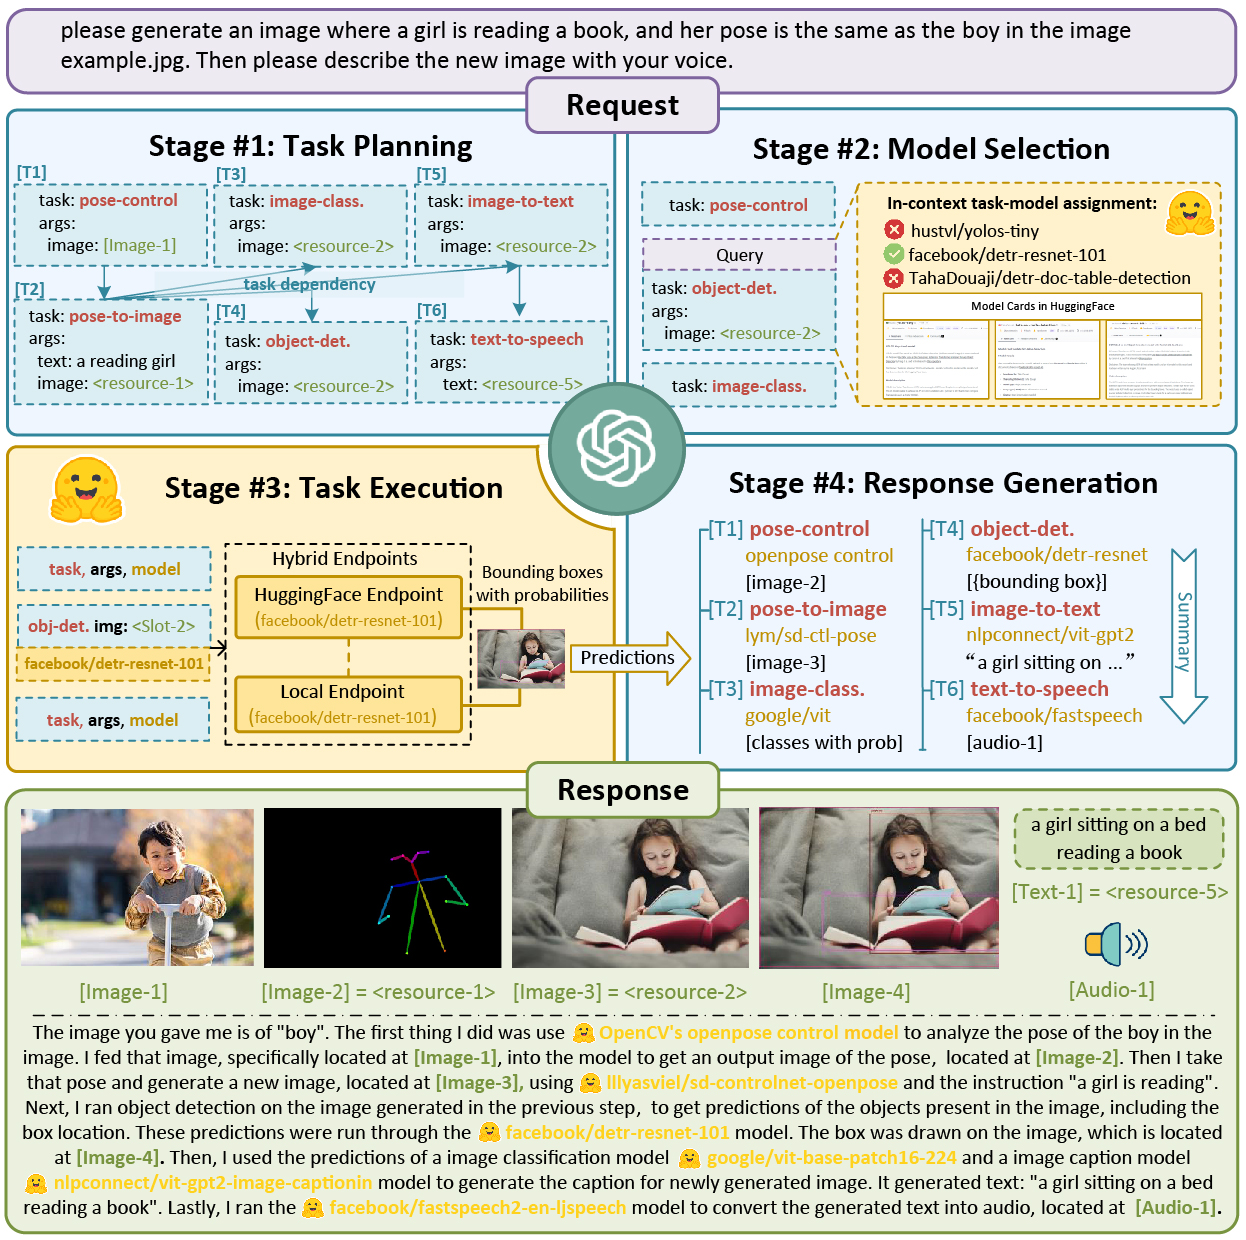
\includegraphics[width=\textwidth, height=\textheight, keepaspectratio]{jarvis_overview}
    \end{center}
\end{figure}
\begin{figure}
    \caption{'JARVIS kan objecten op afbeeldingen herkennen'}
    \begin{center}
        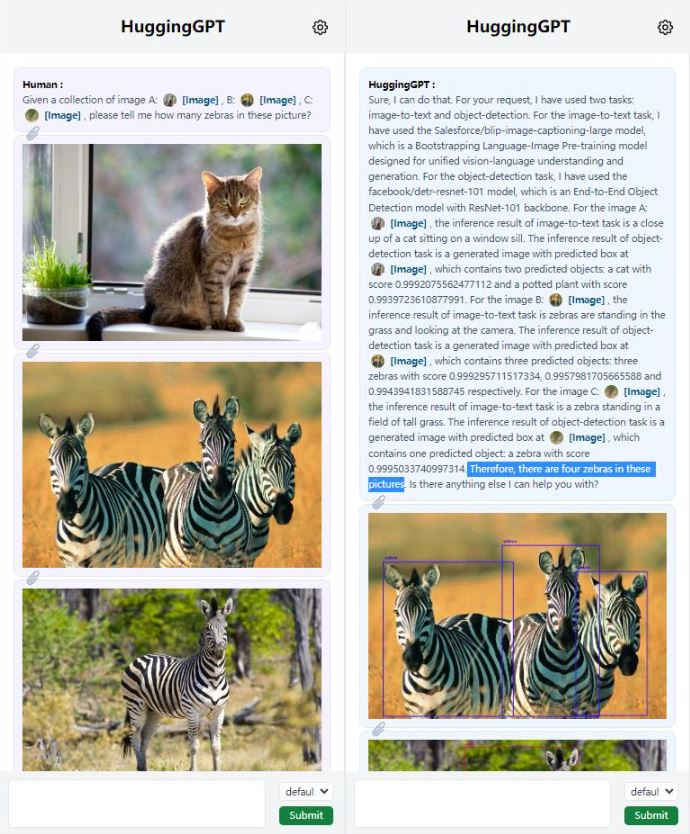
\includegraphics[width=\textwidth, height=\textheight, keepaspectratio]{jarvis_overview_2}
    \end{center}
\end{figure}
\subsection{Elementor AI}
Er zijn talloze manieren om de gebruikerservaring met WordPress voor zowel de programmeurs als eindgebruikers eenvoudiger te maken. Een voorbeeld hiervan is Elementor. Het bedrijf staat o.a. bekend voor WordPress hosting, een builder om websites te maken en hun plugin die websites met een Elementor thema visueel kan aanpassen.
\\\\
Op 3 april 2023 bracht Elementor een tweede Roadmap Event \autocite{Laster2023} uit waar ze hun Elementor AI voorstelden. Het is in staat om tekst te vertalen in code en kan gebruikt worden om elementen aan te passen zonder enige programmeerkennis. Veel meer extra informatie over functionaliteiten en prijzen zijn er op moment van schrijven nog niet over terug te vinden.
\subsection{Auto-GPT}
Het project \href{https://github.com/Significant-Gravitas/Auto-GPT}{Auto-GPT: An Autonomous GPT-4 Experiment} is op GitHub raadpleegbaar en is op moment van schrijven nog een experiment. De laatste demo is momenteel van 16 april 2023 waarin de tool een webpagina analyseert om een samenvatting van de inhoud te maken en op te slaan in een tekstbestand.
\\\\
Een mogelijke toepassing van deze tool is het analyseren van een reeds bestaande webshop en de inhoud ervan in code teruggeven op een manier dat direct in een bestaand thema kan worden geïmplementeerd.
\subsection{AgentGPT} 
Deze tool is op moment van schrijven nog in beta. Het principe van \href{https://agentgpt.reworkd.ai/nl}{AgentGPT} is simplistisch uitgelegd dat je een complexe opdracht stelt aan de tool, die het vervolgens opdeelt in kleinere taken en elke taak toewijst aan een AI-agent. Die AI-agent krijgt enkel en alleen maar de rechten die hij nodig heeft. Zo kan een agent die iets moet opzoeken bv. geen betalingen uitvoeren. 
\\\\
Sinds begin mei 2023 is het mogelijk om ook eigen taken toe te voegen. Bij de oorspronkelijke release van deze tool was dit nog niet het geval, en was Godmode een alternatief hiervoor. Momenteel lukt het niet om websites volledig te clonen zonder een eigen API-sleutel te voorzien, en bijgevolg te betalen. Het commando “Clone the webshop https://www.coureurlocal.be/” geeft het volgende resultaat:
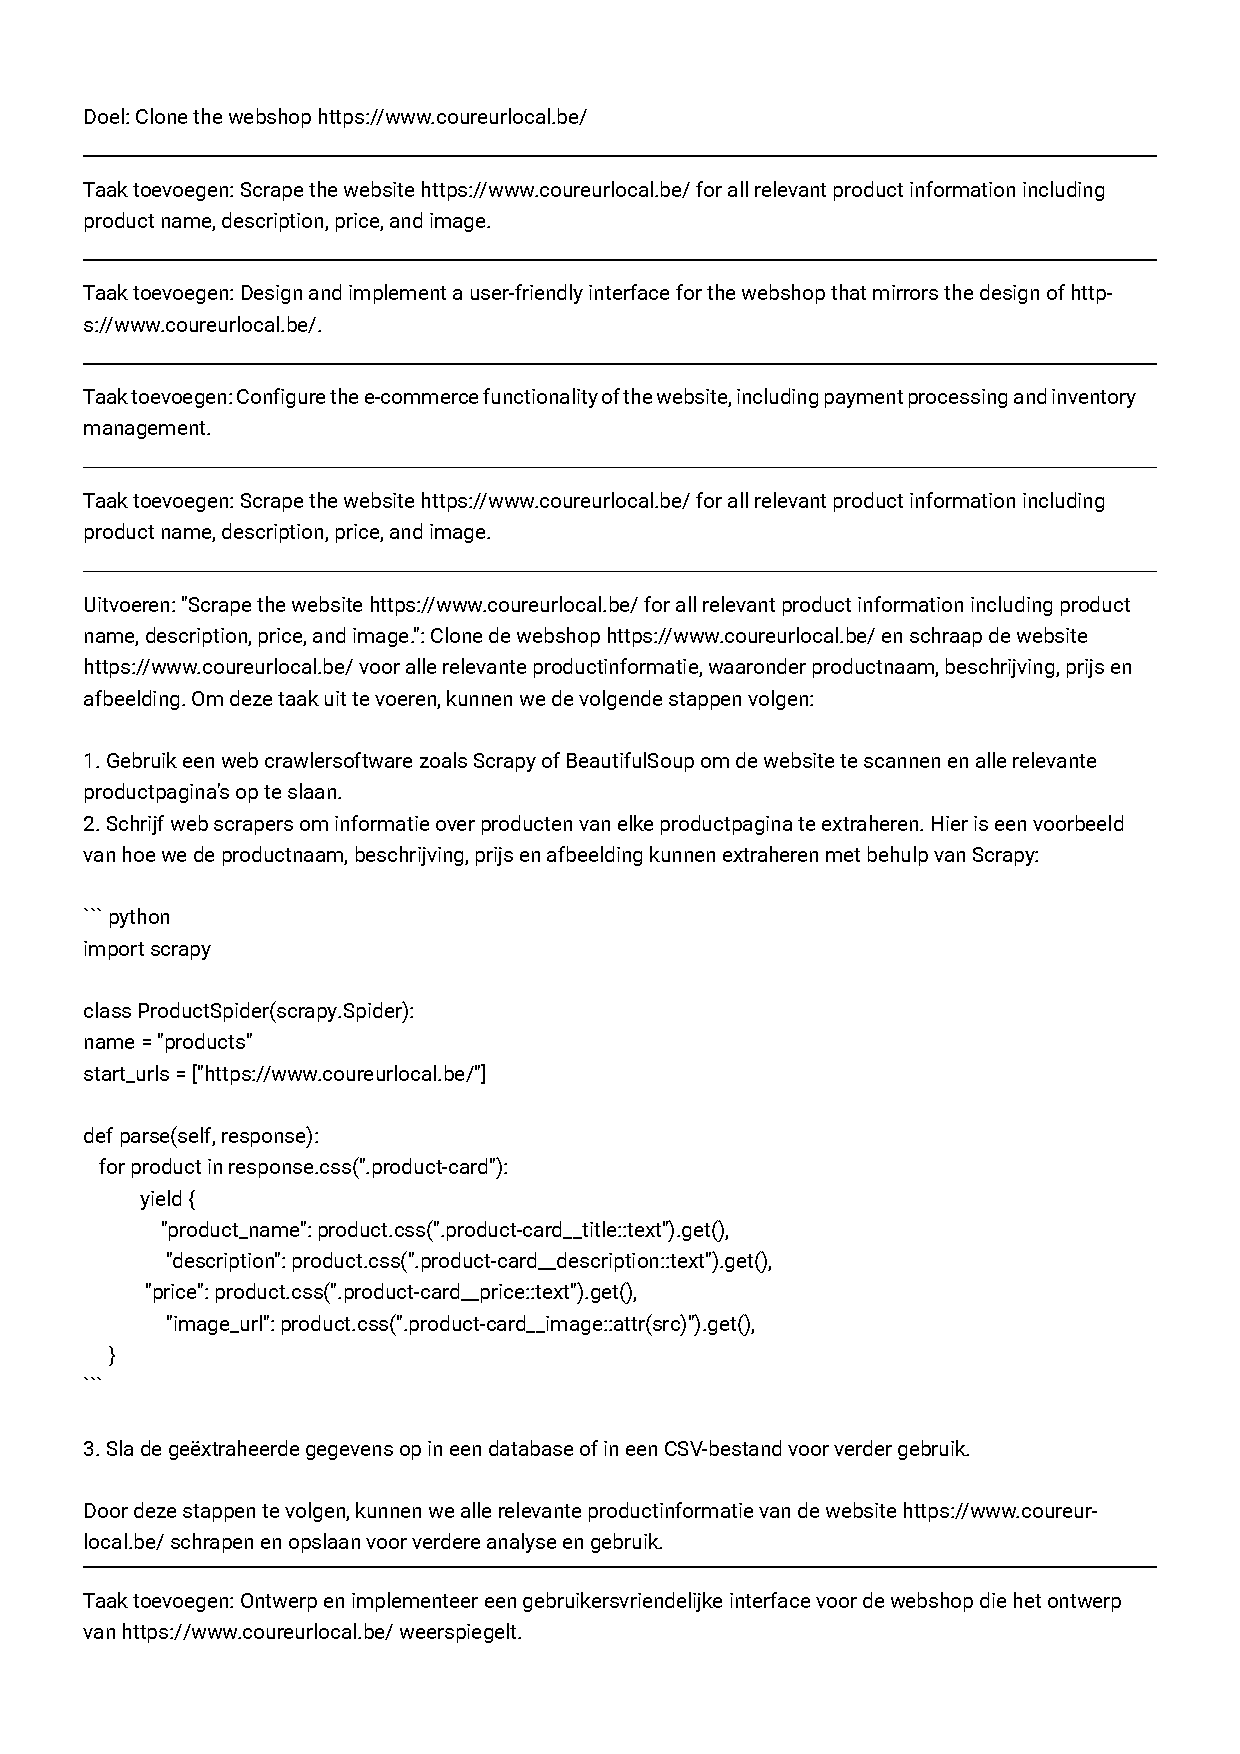
\includepdf[pages=-]{agentGPT_coureur_local.pdf}
\subsection{Godmode}
\href{https://godmode.space}{Godmode} is een alternatief voor AgentGPT dat eerder de mogelijkheid had om zelf taken toe te voegen. De tool laat toe om na elke taak feedback te geven en vereist bijgevolg ook telkens actie van de gebruiker. Uitvoerig gebruik is helaas gratis niet mogelijk en geeft telkens de melding “Due to very high use, please provide your own OpenAI key to continue”. Op moment van schrijven staan \href{https://docs.google.com/forms/d/e/1FAIpQLSdfKYSOEifsbKsfx365zZ0TuZpE9ovLUcAwpGY3NFNRg6l25w/viewform}{inschrijvingen voor Godmode versie 2} open.
\\\\
\subsection{Code Interpreter Plugin}
Dit is een codeer plugin voor ChatGPT waarvan de auteur nog geen toegang heeft verkregen. De plugin biedt ChatGPT een werkende Python-interpreter aan in een sandbox-omgeving. Het zou zelfs in staat zijn om basis video editing te doen en kleine video's te genereren \autocite{Jose2023}.
\section{Webshops}
\subsection{Definitie en belang}
Doorheen de afgelopen jaren zijn webshops en online retail alleen maar in populariteit gestegen \autocite{Roggeveen2020}. Zo was tijdens de coronapandemie, wanneer sociaal contact verboden was, het hebben van een webshop vrij cruciaal. Bedrijven die voornamelijk al een webshop voor Maart 2020 hadden opgesteld genoten het meest van de grote boost in de e-commerce. Het hebben van een webshop geeft daarnaast de mogelijkheid om geen fysieke winkel te moeten starten. Dit kan bijgevolg veel extra kosten te besparen, iets wat voor kleine bedrijven zeer interessant kan zijn \autocite{Beckers2021}.
\\\\
Het is belangrijk dat klanten uitspringen t.o.v. hun concurrenten door verschillende middelen in te zetten op de online markt. Enkel een prijsverschil tonen is niet goed genoeg meer. Daarom is het belangrijk om niet alleen een functionele maar ook een goed verzorgde webshop te hebben \autocite{MatthiasF.Treutner2011}.
\section{CMS}
\subsection{Definitie}
Bij een CMS, afkorting voor contentmanagementsysteem, bepaalt de programmeur in welke mate er wijzigingen kunnen plaatsvinden op een site, zonder dat de klant daarvoor zelf naar de code hoeft te kijken. Via een login systeem kan de klant zelf teksten en afbeeldingen wijzigen, zonder enige hulp van de programmeur. Bovendien kan met behulp van rechten en rollen de klant kiezen om een CMS door verschillende (externe) personen te laten beheren \autocite{Browning2001}.
\subsection{Verband met webshops}
Een webshop heeft als doel goederen en/of diensten te verkopen. Voor een optimale verkoop te garanderen is het cruciaal om zo snel mogelijk te kunnen inspelen op de trends en wijzigingen van de desbetreffende markt. Daarom moet een klant zelf in staat zijn om zijn of haar webshop zelf van inhoud aan te passen, ongeacht zijn of haar technische ervaring. Hiervoor is een CMS een mogelijke oplossing. In plaats van de programmeur extra te betalen voor elke wijziging, kan de klant dit op eigen initiatief aanpassen.
\subsection{Opties}
Vandaag de dag zijn er talloze CMS'en op de markt aanwezig. Team Made, het bedrijf van de co-promotor, heeft de keuze gemaakt om met WordPress te werken. Dit betekent niet dat WordPress dan ook de beste keuze is. Afhankelijk van project tot project, en de eigen programmeerervaringen, moet een afweging worden gemaakt welke CMS het beste uit komt.
\\\\
Er zijn niet veel uitgebreide vergelijkende studies terug te vinden over de verschillende CMS'en. In een studie van 2011 blijkt dat op basis van verschillende aspecten zoals het aantal installaties en het aantal online zoekresultaten, dat Joomla, Drupal en WordPress de meeste efficiënte CMS'en zijn \autocite{Patel2011}. Ook in een studie van 2018 die meer de technische aspecten bekeek, waren dit de meest populaire open-source CMS'en \autocite{MartinezCaro2018}.
\subsection{Uitbreidingen}
Niet elke CMS is even flexibel wanneer het over uitbreidingen gaat. Zo is WordPress ontworpen voor blogwebsites te maken en is standaard niet in staat om als webshop te functioneren. Dit is waar plugins zoals WooCommerce, een open-source e-commerce plugin, van pas komen. Daarnaast laat WordPress custom (eigen geschreven) code toe om de functionaliteiten uit te breiden. 
\subsection{Beperkingen}
Om een CMS te onderhouden, denk aan toekomstig gebruik, is het noodzakelijk om enige technische achtergrond te hebben. Het hangt zowel van de leercurve van de webdeveloper zelf als van de complexiteit van een CMS af hoelang het duurt eer de webdeveloper een CMS onder de knie heeft \autocite{DriesBlanchaert2022}.
\\\\
Afhankelijk van de noden en wensen van de klant, het type webshop, het assortiment aan producten... kan het gebruik van professionele afbeeldingen voor een webshop belangrijk zijn. Deze hebben een groter formaat en bijgevolg ook meer opslagruimte nodig. Het is aan de webdeveloper om dit in het achterhoofd te houden bij het kiezen van een CMS. Mogelijke oplossingen hiervoor zijn een automatische compressie toepassen of een limiet van bestandsgrootte te implementeren in het programma. \autocite{LatumenRonaldDekker2004}

\section{Overname webshops}
De co-promotor wenst sneller webshops te kunnen overnemen binnen zijn bedrijfstermen, ongeacht de werkwijze hiervoor. Het belangrijkste is een werkend resultaat dat hij en zijn medewerkers kunnen beheren. Hoe meer van het proces geautomatiseerd is, hoe minder manueel werk nodig is en bijgevolg hoe sneller een overname kan afgerond worden.
\subsection{Automatisatie}
Er zijn heel veel online tools terug te vinden die de broncode van een website of webshop kunnen downloaden. Een aantal voorbeelden hiervan zijn: HTTrack, GNU Wget, SiteSucker, Teleport Pro enzovoort. Ook voor het exporteren van data die via een plugin worden gegenereerd, zijn een hele hoop alternatieve plugins beschikbaar. Een bekend voorbeeld daarvan voor WordPress is BackWPup. Het grote probleem hierbij is dat veel tools, na persoonlijk testen, niet alle data kunnen bemachtigen. Daarbovenop is nog steeds enige technische achtergrond vereist om met deze data effectief aan de slag te kunnen gaan.  
\subsection{Bijkomende aspecten}
Niet elk contentmanagementsysteem is standaard voorzien van trackingtools om het gedrag van de gebruikers te analyseren. Afhankelijk van de opdracht van de klant, kan dit wel een noodzakelijke behoefte zijn die ergens in het programma moet worden geïmplementeerd. \autocite{DeBruijn2013}
\\\\
Een andere belangrijke factor is de beveiliging. Het is aan de webdeveloper zelf om hier alert in te zijn door bv. enkel betrouwbare plugins te installeren die goed onderhouden zijn. Dit onderzoek zal moeten bepalen of dit kan geïmplementeerd worden door gebruik te maken van AI-tools of dat dit best manueel werk blijft. \autocite{Bottelbergs2013}   
\subsection{Beperkingen}
Het overnemen van een webshop komt niet zonder beperkingen kijken. Afhankelijk van wat in de privacy of terms (ToS) beschreven staat op een webshop, is niet alle data zomaar gratis over te nemen. Helaas worden ToS'en vaak nog over het hoofd gezien door zowel de consument als het bedrijf \autocite{Braun2019}.  
\\\\
Bij een analyse over de verkregen webshops van de co-promotor zijn bij veel webshops een aantal kleine fouten teruggevonden. Zo zijn niet alle menubalken responsief en zijn bepaalde elementen zoals de back-to-top-button (een knop die de gebruiker terug naar boven brengt) niet altijd even goed zichtbaar. Deze fouten moeten uiteraard niet overgenomen worden, of indien mogelijk worden aangepast.  

\section{Huidige trends}
\subsection{AI is booming}
Op moment van schrijven is AI de wereld aan het overnemen en heeft dit bijgevolg grote invloed op deze paper. Zo worden er elke dag nieuwe AI-tools op de markt gebracht. Momenteel is ChatGPT, een chatbot ontwikkeld door OpenAI, wereldwijd de bekendste AI-tool. Deze chatbot had maar liefst twee maanden nodig om 100 miljoen gebruikers te bereiken \autocite{Brownlee2023}. Het heeft momenteel nog steeds wereldwijd een grote impact en is dagelijks in het nieuws. Het brengt ook heel vele ethische vragen omtrent het gebruik ervan met zich mee. Zo is het mogelijk om de chatbot code te laten generen, of zelfs thesissen volledig te laten schrijven \autocite{Dumitrescu2023}.
\\\\
Veel mensen en bedrijven, waaronder Meta, waren eind 2022 nog van mening dat Augmented Reality de volgende grote evolutie binnen de IT-wereld ging worden \autocite{Brownlee2023a}. Zij zagen deze AI-trend net zoals velen niet aankomen en moesten noodgedwongen openstaande projecten laten vallen om mee te kunnen met hun concurrenten. Zo wilt Meta zich nu focussen op hun producten met AI te voorzien en laten ze de Metaverse bijgevolg (even) opzij \autocite{Howley2023}. Ook Microsoft is volop bezig met AI in hun volledige Office 365 te integreren \autocite{Hendrikman2023}. 
\subsection{Verschillende types AI}
AI bestaat al een tijdje in verschillende vormen. Het is pas in Januari 2021, dat OpenAI hun product Dall-E lanceerde en AI echt in populariteit is gerezen. Zo zijn er naast Dall-E ook nog AI-tools die automatisch afbeeldingen kunnen genereren zoals Hotpot.ai, stemmen vervormen zoals voice.ai, video's genereren zoals Synthesia.io enzovoort. Een paar maand later heeft OpenAI ChatGPT uitgebracht \autocite{Bridle2023}.
\\\\
Voor deze paper zullen we ons focussen op AI-tools zoals ChatGPT omdat deze code kunnen genereren. Wat AI-tools zoals ChatGPT nog interessanter maken is dat ze multimodal large language models zijn, wat betekent dat ze zowel met tekst als afbeeldingen kunnen omgaan. Dit is zeer interessant en mogelijks een handig middel voor een webshop overname te doen versnellen \autocite{MelissaHeikkilaea2022}.
\subsection{Limieten en pijnpunten}
Foute informatie verkrijgen is geen uitzondering. Zo worden zelfs tijdens live-demonstraties van Bing foute brongegevens verspreidt \autocite{Bellens2023}. Je moet als gebruiker heel goed opletten wat je met de verkregen informatie gaat doen, en altijd zeker op feiten controleren. Het is als eindgebruiker van deze tools heel erg verleidelijk om de verkregen resultaten als volledig accuraat te beschouwen.
\\\\
Op vlak van functionaliteit komen veel AI-tools nog met grote beperkingen met zich mee. Doordat de grote AI-golf tijdens het schrijven van deze bachelorproef is ontstaan, zijn nog veel tools in beta zoals Bing AI \autocite{Dent2023}, of nog niet overal publiek toegankelijk zoals Google's Bard \autocite{Dawes2023}. Omdat deze AI-tools zodanig populair zijn, liggen de servers vaak door groot gebruik ook plat, zijn ze tijdelijk onbeschikbaar of worden antwoorden heel erg traag gegenereerd \autocite{Leong2023}. 
\\\\
Een groot limiet dat ChatGPT bij release had was dat alle data waarop dit model getraind was tot en met 2021 geldig was. De chatbot was niet in staat om gegevens van het internet op te halen, en bijgevolg informatie over nieuwere gebeurtenissen te bekomen. Daarnaast moet de gebruiker nog steeds zelf zeer specifiek zijn in het opstellen van een vraag, of blijven doorvragen tot een gewenst antwoord is bekomen \autocite{Tips2022}. Complexere vragen zijn op moment van schrijven nog niet mogelijk om aan ChatGPT te stellen.
\\\\
Een kleine update: sinds de ChatGPT versie van 3 mei is het wel mogelijk om complexere scripten te laten genereren zoals 'Schrijf mij een script uit dat WordPress met WooCommerce opstelt'. Helaas zijn deze nog niet volledig op punt en kunnen er grote schrijffouten aanwezig zijn. Soms kan de chatbot ook geen zin hebben (zie figuur 2.1).
\begin{figure}
    \caption{'ChatGPT kan niet altijd een script genereren'}
    \begin{center}
        
\includegraphics{chatgpt_wordpressWithWooCommerceScript}
    \end{center}
\end{figure}
\\\\
Bepaalde AI-tools zoals 10Web bieden de mogelijkheid aan om websites volledig over te nemen, maar zijn vastgebonden aan één of meerdere prijsabonnementen. Daarnaast is het niet altijd direct duidelijk wat je voor een bepaalde prijs krijgt wegens zeer vage omschrijvingen op de website, en of het verkregen resultaat (een overgenomen webshop) kan geëxporteerd worden buiten de omgeving van de AI-tool. Vermoedelijk zijn dit bewuste keuzes om klanten te lokken.  

\subsection{Tijdelijke oplossingen}
Steeds meer en meer bedrijven zoals Expedia en Instacart werken nauw samen met OpenAI om ChatGPT van \href{https://openai.com/blog/chatgpt-plugins}{plugins} te voorzien. Hiermee is de chatbot (in beperkte mate) in staat om (recente) informatie van het web op te halen. Dit opent heel wat mogelijkheden, maar brengt bijgevolg ook veel bezorgdheid omtrent data en privacy met zich mee \autocite{WillKnight2023}. Tijdens het verloop van de literatuurstudie heeft de auteur geen enkele toegang verkregen tot één van deze plugins.
